\documentclass[tikz]{standalone}
\usetikzlibrary{shapes.geometric}    % trapezium
\usetikzlibrary{arrows}              % arrow tips
\usepackage{amsmath, amsfonts}
\usepackage{bm}                      % boldsymbol
\usepackage{makecell}                % makecell
\usetikzlibrary{matrix,calc}
\usepackage{color}
\usepackage{xcolor}
\definecolor{mygray}{HTML}{F0F0F0}
\definecolor{myred}{HTML}{CD594A} 
\definecolor{mygreen}{HTML}{829356} 
\definecolor{myblue}{HTML}{3C6478} 
\usepackage{mathtools}
\usetikzlibrary{decorations.pathreplacing}

\newcommand{\trans}{\text{T}}
\newcommand{\inv}{{-1}}
\newcommand{\eins}{\mathds{1}}
\DeclareMathOperator{\E}{\mathbb{E}}
\DeclareMathOperator{\I}{\mathbb{I}}
\newcommand{\tbf}[1]{\textbf{#1}}
\DeclareMathOperator{\tr}{tr}
\newcommand{\D}{\mathbf{D}}
\newcommand{\K}{\mathbf{K}}
\begin{document}


\definecolor{mygray}{HTML}{F0F0F0}
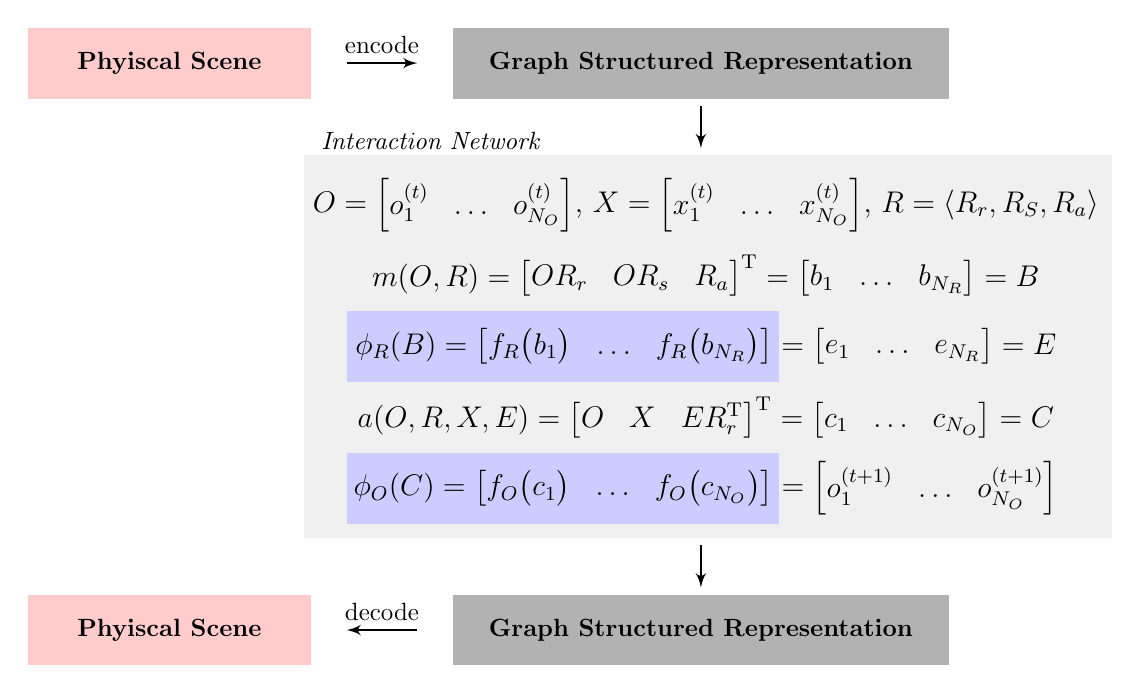
\begin{tikzpicture}[>=latex',thick, scale=0.9, every node/.style={scale=0.9}]] 
  % \node [draw, rectangle, minimum size=5pt, fill=blue!40, color=blue!20, name=AND]
  % at (0,0) {AD}; 

  \draw [fill=red!20, draw=none] (-6,0) rectangle (-2,1) node[pos=.5]
  {\textbf{Phyiscal Scene}};

  \draw [fill=gray!60, draw=none] (0,0) rectangle (7,1) node[pos=.5]
  {\textbf{Graph Structured Representation}};

  \draw [->] (-1.5, 0.5) -- node [above] {encode} (-0.5, 0.5); 

  \draw [->] (3.5, -0.1) -- node [right] {} (3.5, -0.7); %extract/apply

  \node at (-0.3, -0.6) {\emph{Interaction Network}};

  \draw [fill=mygray, draw=none] (-2.1, -0.8) rectangle (9.3, -6.2);

  \node at (3.5, -1.5) {\large{
      $O = \begin{bmatrix} o_1^{(t)} & \dots & o_{N_O}^{(t)} \end{bmatrix}$,
      $X = \begin{bmatrix} x_1^{(t)} & \dots & x_{N_O}^{(t)} \end{bmatrix}$,
      $R = \langle R_r, R_S, R_a \rangle$
    }};

  \node at (3.5, -2.5) {\large{
      $m(O, R) = \begin{bmatrix} O R_r & OR_s & R_a \end{bmatrix}^\trans =
      \begin{bmatrix} b_1 & \dots & b_{N_R} \end{bmatrix} = B $
    }};

  \draw [fill=blue!20, draw=none, label={NN}] (-1.5,-4) rectangle (4.6, -3);

  \node at (3.5, -3.5) {\large{
      $\phi_R(B) =
      \begin{bmatrix} f_R \big(b_1\big) & \dots & f_R \big(b_{N_R}\big) \end{bmatrix}
      = \begin{bmatrix} e_1 & \dots & e_{N_R}\end{bmatrix} = E$
    }};

  \node at (3.5, -4.5) {\large{
      $a(O, R, X, E) = \begin{bmatrix} O & X & E R_r^\trans \end{bmatrix}^\trans =
      \begin{bmatrix} c_1 & \dots & c_{N_O} \end{bmatrix} = C $
    }};

  \draw [fill=blue!20, draw=none, label={NN}] (-1.5,-5) rectangle (4.6, -6);

  \node at (3.5, -5.5) {\large{
      $\phi_O (C) =
      \begin{bmatrix} f_O \big( c_1 \big) & \dots & f_O \big( c_{N_O} \big) \end{bmatrix}=
      \begin{bmatrix} o_1^{(t+1)} & \dots & o_{N_O}^{(t+1)} \end{bmatrix}$
    }};

  
  \draw [->] (3.5, -6.3) -- node [right] {} (3.5, -6.9); % update

  \draw [fill=gray!60, draw=none] (0,-7) rectangle (7,-8) node[pos=.5]
  {\textbf{Graph Structured Representation}};

  \draw [fill=red!20, draw=none] (-6,-7) rectangle (-2,-8) node[pos=.5]
  {\textbf{Phyiscal Scene}};

  \draw [<-] (-1.5, -7.5) -- node [above] {decode} (-0.5, -7.5); 
  
  
\end{tikzpicture}
\end{document}
